\chapter{System Design}\label{chap:system_design}
%chapter that includes other parts. Then gives a tail describing how we the report is structured
%Describe when theory is introduced in each sprint. Describe how sprint chapter is structured.
\chapter{Introduction}
%Describes the premise of the project. That we collaborate and they come with requirements and what they want overall. 
This project has been made in collaboration with Mariendal IT.
They specialize in IT and offer services such as hosting, security, and operations management\cite{Mariendal_OmOs}.
As stakeholders, they have provided insight towards their perceived requirements, users to perform evaluation, and feedback regarding the developed product.
%their problem

While accommodating customers and users of their systems, it is often necessary to arrange meetings.
Their current system for booking meeting rooms is insufficient for their use, as they do not integrate well with the systems they already use.
Therefore they are looking for a new solutions that accommodates their needs when booking either spontaneous or planned meetings. 
%current tools are insufficient due to not being able to see if already in use, 
Henceforth, Mariendal IT will be referred to as the stakeholder. 


We decided to develop a mobile application to create a system that can implement the fingerprinting technique in a suitable way.
The benefit of using a mobile application is that typical mobile devices already have the capability to interact and collect data from Bluetooth devices, such as Bluetooth beacons. 
This allowed us to integrate the process of collecting the data, doing classification, and applying the resulting classification model to conduct experiments within the same system.

A primary function of the application is to collect data from the aforementioned beacons. 
As illustrated in figure \ref{fig:ScanAdvertisement}, when the device is running, it will scan for advertisement packets broadcast by the Bluetooth beacons.

\begin{figure}[H]
    \centering
    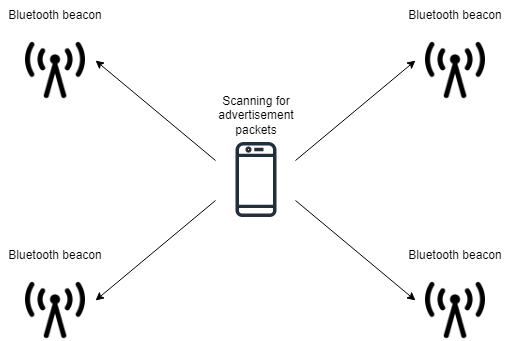
\includegraphics[width=0.5\textwidth]{images/ScanningForAdvertisement.drawio.png}
    \caption{Illustrating a mobile device scanning for Bluetooth beacons}
    \label{fig:ScanAdvertisement}
\end{figure}

Each beacon broadcasts data, which may include a unique identifier for the specific beacon or manufacturer-specific information.
A device configured to receive these broadcasts can extract this information and also calculate the received signal strength indicator (RSSI) of the signal.

As outlined in section \ref{sec:fingerprinting}, fingerprinting involves two stages.
The first stage entails the generation of a map based on the RSSI of the received Bluetooth signal. The second stage involves estimating the unknown location of a Bluetooth receiver.

Through the collection of the broadcast data from the beacons, the application supports the initial phase of fingerprinting, which involves map generation.
Figure \ref{fig:CreateMap} illustrates the map generation process. During this process, a device equipped with the application collects data while being carried around the room in a specific pattern.

Moreover, the beacons are strategically positioned to demarcate the room's perimeter, a critical aspect in the second stage, which entails position inference.

\begin{figure}[H]
    \centering
    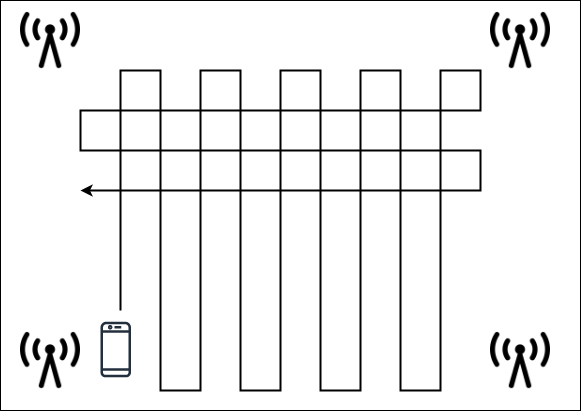
\includegraphics[width=0.5\textwidth]{images/CreateMap.drawio.png}
    \caption{Illustrating a mobile device collecting data from Bluetooth beacons}
    \label{fig:CreateMap}
\end{figure}

To support the second phase of fingerprinting, we have developed a classification module as part of the application. 
By collecting new data and using the map generated during the first phase, the classification module is able to classify the position of other devices relative to the room. 
Using the classifier, the application is able to estimate whether a device is either inside or outside the room.


% Intro text - from data collection, but rewrite.
% Explain the overall design for the data collection phase by using diagrams of central components (DataCollector, etc.)
% Deep-dive into various aspects of the implementation, relying on the diagrams to explain the overall design

\section{Phase one: Data collection}\label{sec:first_phase}
As the quality of the system is reliant on the accuracy and precision of the map during this phase it is critical to create a map of high quality.
Therefore, steps must be taken to ensure this quality. 
\citeauthor{improving_indoor_localization}~\cite{improving_indoor_localization} suggests that measurements be taken by systematically partitioning the area in a grid and then performing measurements for each cell of the grid for n-seconds. 
We propose a design where, instead of having a fixed collection time, a fixed minimum number of measurements is received from each beacon.
We do this, as beacons broadcast on a fixed time-schedule \cite{apple2023ibeacon}.
This is done to ensure that all beacons have a representative set of measurements with low standard deviation when constructing the map.
To ensure a low standard deviation, we use the following procedure.
Data is collected from each beacon until a minimum number of data points are collected, and a  satisfiable standard deviation is reached.
As fluctuations can cause large deviations in the collected data, the data collection for a beacon is halted as soon as the prior condition is satisfied.
The average RSSI value from the collected measurements from the beacons is used to create entries for the map.
During the measurement collection each cell is labelled as being either inside or outside of the meeting room.
This process is repeated for each cell in the grid to construct the entries for the map. 




% use this as reference for the following sections, as we base our implementation on this
% data class - contains structured parses of the data we receive from the beacons
\subsection{Parsing Beacon Advertisement Packet Data}

As previously mentioned, we use Bluetooth Low Energy beacons that broadcast specific advertisement packets which can be perceived by other nearby devices.
The key element of these packets is a particular sequence of bytes encapsulating valuable information about the beacon and its broadcast. 
In this section, we delve into the details of this byte stream and present an analytical dissection of \texttt{KBeaconData}, a wrapper class whose purpose is to interpret and abstract over the byte stream.

\subsubsection{Beacon Advertisement Packet Structure}
% 4C-00-02-15-77-77-77-2E-6B-6B-6D-63-6E-2E-63-6F-6D-00-00-01-00-03-39-2B-C5
% Company ID:  4C-00
% Beacon type: 02-15
% UUID:        77-77-77-2E-6B-6B-6D-63-6E-2E-63-6F-6D-00-00-01
% Minor:       39-2B
% Major:       00-03
% TxPower:     C5
	 
Each beacon advertisement packet consists of a string of 25 bytes.
These bytes are distributed in a specific order, serving as unique identifiers and providing a variety of information about the beacon. 
The given byte stream is an example of an advertisement and can be represented as a sequence of hexadecimal values:


\noindent\texttt{4C-00-02-15-77-77-77-2E-6B-6B-6D-63-6E-2E-63-6F-6D-00-00-}


\noindent\texttt{00-03-39-2B-C5}


The allocation of bytes is as follows:

\begin{itemize}
  \item The initial two bytes, known as the Company ID (e.g., \texttt{4C-00}, i.e. Apple), uniquely identify the company that created the specification for the beacon.
  \item The next two bytes, known as the beacon type, represents the type of the beacon. For proximity beacons, like the ones we use, these two bytes must be set to \texttt{02-15}.
  \item The subsequent 16 bytes represent the \textit{Universally Unique Identifier} (UUID).
This UUID (e.g., \texttt{77-77-77-2E-6B-6B-6D-63-6E-2E-63-6F-6D-00-00-01}) is a standard identifier that the beacon broadcasts, allowing the receiving devices to recognize the specific beacon or a group of beacons.
  \item The next two bytes denote the Major number (e.g., \texttt{00-03}), and the two bytes following them indicate the Minor number (e.g., \texttt{39-2B}).
These two values allow further differentiation among beacons.
  \item The final byte, called TxPower (e.g., \texttt{C5}), indicates the \textit{Measured Power}, which represents a standardized signal strength value within Apple's proximity beacon technology. Obtained via a systematic procedure using an iPhone 5s, it involves sampling the Received Signal Strength Indicator (RSSI) from the beacon at a one-meter distance. Outliers in the RSSI samples are discarded to minimize signal strength variability. The remaining data is averaged, producing the 'Measured Power' - a benchmark for subsequent ranging calculations.
\end{itemize}
\cite{apple2023ibeacon}

\subsubsection{Role of the KBeaconData Class}

The KBeaconData class is designed to parse and encapsulate the information embedded within the beacon advertisement packet.
As a wrapper class, it takes a byte array as an input and decodes the values, storing them in properties for subsequent use.
The implementation can be seen in code snippet \ref{lst:KBeaconData}.



\begin{figure}[H]
\begin{lstlisting}[
	language=CSharp, 
	frame=single, 
	label={lst:KBeaconData},
	caption={C\# Implementation of the KBeaconData Class for processing Bluetooth Low Energy (BLE) Beacon Advertising Packets}, 
	captionpos=b] 
public sealed class KBeaconData {
	private const int ByteCount = 25;

	public Guid Uuid { get; }

	public byte[] CompanyId { get; }

	public ushort Major { get; }
	public ushort Minor { get; }

	public sbyte TxPower { get; }

	public KBeaconData(byte[] data) 
		: this(data, BitConverter.IsLittleEndian) { }

	public KBeaconData(byte[] data, bool isLittleEndian) {
		if (data.Length != ByteCount)
			throw new ArgumentException($"Number of bytes was {data.Length}, expected {ByteCount}.");

		if (isLittleEndian) {
			CompanyId = data.Take(2).ToArray();
			Uuid = new Guid(
				BitConverter.ToInt32(data.Skip(4).Take(4).ToArray()),
				BitConverter.ToInt16(data.Skip(8).Take(2).ToArray()),
				BitConverter.ToInt16(data.Skip(10).Take(2).ToArray()),
				data.Skip(12).Take(8).ToArray()
			);
			Major = BitConverter.ToUInt16(data.Skip(20).Take(2).ToArray());
			Minor = BitConverter.ToUInt16(data.Skip(22).Take(2).ToArray());
		} else {
			CompanyId = data.Take(2).ToArray();
			Uuid = new Guid(
				BitConverter.ToInt32(data.Skip(4).Take(4).Reverse().ToArray()),
				BitConverter.ToInt16(data.Skip(8).Take(2).Reverse().ToArray()),
				BitConverter.ToInt16(data.Skip(10).Take(2).Reverse().ToArray()),
				data.Skip(12).Take(8).ToArray()
			);
			Major = BitConverter.ToUInt16(
				data.Skip(20).Take(2).Reverse().ToArray()
			);
			Minor = BitConverter.ToUInt16(
				data.Skip(22).Take(2).Reverse().ToArray()
			);
		}
		TxPower = (sbyte)data[^1];
	}
}
\end{lstlisting}
\end{figure}

The notion of endianness is crucial while interpreting the byte sequence.
It refers to the byte order in which the integers are stored in the computer memory. In the context of the KBeaconData class, the constructor accepts a boolean parameter that indicates whether the byte order of the data is little-endian or not. If the byte order is indeed little-endian, the sequence is read as-is. Otherwise, the sequence is reversed before interpreting, thereby maintaining the accuracy of the parsed data.

In both little and big-endian scenarios, the first two bytes are extracted as the Company ID.
However, the remaining data is parsed differently depending on the endianness. If the byte order is little-endian, the bytes are sequentially processed. The UUID is constructed from the next 16 bytes, with the first four bytes converted to an integer, the next four bytes to two short integers, and the last eight bytes remain as a byte array. The Major and Minor values are derived from the next two bytes each, interpreted as unsigned short integers. In case of big-endian, the sequence is reversed before parsing the UUID, Major, and Minor values.

The last byte, regardless of the endianness, is directly converted to a signed byte to represent the TxPower.


The KBeaconData class thereby provides an effecient way to parse, encapsulate, and interpret the data from beacon advertisement packets.

\subsubsection{Testing the KBeaconData class}
Unit testing is a vital element within the larger framework of software testing. 
As the name suggests, it focuses on testing individual units of code, traditionally functions or methods, to ascertain their robustness and correctness. By isolating each part of the software, it enables developers to verify the correctness of their code at a granular level, ensuring that each component functions as expected.\cite{sommervilleSoftwareEngineering2016}

This method of testing carries numerous benefits, primarily improving the design, enhancing maintainability, and facilitating the refactoring of code. It significantly simplifies the debugging process, as it allows for easy identification of issues at the unit level rather than in a composite system. Moreover, it fosters the evolution of software by making it more resilient to changes, as potential issues can be mitigated before they propagate through the system.\cite{sommervilleSoftwareEngineering2016}

We use the xUnit.net testing framework for .NET, which provides a comprehensive and extensible set of testing tools. This framework simplifies the creation of test cases, supports parallel test execution, and integrates seamlessly with various development environments.\cite{xunitdotnet}

In the context of the KBeaconData class, we have designed several unit tests to validate its functionality. The tests focus on different aspects of the class, such as the correct parsing of beacon advertisement packet data, the handling of endianness, and the proper handling of invalid input data. 

We initially test the KBeaconData class constructor using both little-endian and big-endian test data. These tests ensure that the class correctly interprets data irrespective of the byte order. We examine the resulting UUID, Major, Minor, TxPower, and CompanyId values, asserting their equality to the expected values.

Subsequently, we test the class for its ability to handle invalid data. We attempt to construct a KBeaconData object with data arrays of insufficient length and null arrays. In line with best practices, we anticipate the class to throw an ArgumentException in the former scenario, indicating an inappropriate data array length, and an ArgumentNullException in the latter scenario, indicating the absence of data.

Lastly, we perform an equality test between the CompanyId values of a KBeaconData object created with little-endian data and a KBeaconData object created with big-endian data. As the CompanyId should remain consistent regardless of byte order, this test verifies the byte order independence of the CompanyId.

Code snippet \ref{lst:KBeaconDataTest} shows an example of a unit test which validates the correct parsing of beacon advertisement data in the little-endian format, asserting that the extracted UUID, Company ID, Major, Minor, and TxPower values match the expected results.

\begin{figure}[H]
\begin{lstlisting}[
	language=CSharp, 
	frame=single, 
	label={lst:KBeaconDataTest},
	caption={An example of a unit test for \texttt{KBeaconData}, testing the correctness of parsing data in the little endian format}, 
	captionpos=b] 
private const sbyte ExpectedTxPower = 0x16;
	
private readonly byte[] testData = { 
	0x06, 0x17, 0x9C, 0xAA, 0xB5, 0xF3, 0x7E, 0x78, 0x26, 0xD3, 0xCD, 0x82,
	0xE3, 0x03, 0xDE, 0xCD, 0x5D, 0x3A, 0xDE, 0xF4, 0xA9, 0x96, 0xD9, 0x23, 
	0x16 
};

[Fact]
public void TestConstructor_testData_LittleEndian() {
	const ushort expectedMinor = 0x23D9;
	const ushort expectedMajor = 0x96A9;

	byte[] expectedCompanyId = { 0x06, 0x17 };

	Guid expectedUuid = new("787ef3b5-d326-82cd-e303-decd5d3adef4");
	KBeaconData kBeaconData = new(testData, isLittleEndian: true);

	Assert.Equal(expectedUuid, kBeaconData.Uuid);
	Assert.Equal(expectedCompanyId, kBeaconData.CompanyId);
	Assert.Equal(expectedMajor, kBeaconData.Major);
	Assert.Equal(expectedMinor, kBeaconData.Minor);
	Assert.Equal(ExpectedTxPower, kBeaconData.TxPower);
}
\end{lstlisting}
\end{figure}

% overall section to describe the implementation of the data collection system
% uses system diagram & frontend  as reference, along with selected code snippets
% to explain the system implementation
\subsection{Data Collection Implementation}\label{sec:data_collection_implementation}
This section presents an an overview of the system architecture and data flow.

Figure~\ref{fig:implementation_diagram} shows the overall system architecture and data flow.
We implictly assume usage of the previously described \texttt{KBeaconData} class throughout the program flow, however we have omitted it from the diagram in the interest of keeping the overview concise and comprehensible.

The system is largely event-driven, which helps decouple the system components. 
Therefore, much of the responsibility of the \texttt{Controller}, shown in Figure~\ref{fig:implementation_diagram}, is to subscribe services to events and to handle the events when they are raised thus delegating responsibility across components. 

When the application starts, the \texttt{Beacon Scanner} component will begin listening for Bluetooth devices and add those who match the iBeacon signature to a list of devices.
These devices are shown to the user in the view inside of a list.
Each device in the list has a corresponding toggle, letting the user select which devices to use for data collection.
After selecting at least one device, the user can click the "Start listening collection" button, which prompts the \texttt{Data Collector} class to listen for advertisement packets from the selected devices, facilitated through the \texttt{Advertisement Scanner} component. 
While the \texttt{Data Collector} is actively receiving packets from the \texttt{Advertisement Scanner}, the \texttt{BeaconRssis} hashtable is continuously populated with the selected beacons' GUIDs and latest RSSI values.


At this point, the data collection process for a given point in the grid may begin.
First, the user must select a label (inside or outside), denoting whether the current point is within or outside the room.
Then, when the user presses the "Collect data" button on the view, the \texttt{Data Collector} class will begin collecting data from the selected beacons.
The data collection process is implemented using standard deviation to account for fluctations.
During data collection, the latest beacon RSSI measurements are added to a collection every 500ms until at least 40 measurements have been made, and the standard deviation is lower than some preset threshold.
The collection interval was selected based on a heuristic: the beacons advertise every 100ms, and therefore 500ms was selected to account for potential delays.
Originally, the threshold was set to 20 measurements based on \citeauthor{improving_indoor_localization}~\cite{improving_indoor_localization}, which collected data for 10 seconds.
Since we collect a measurement every 500ms, we collect 20 measurements in approximately 10 seconds. However, during development, we found that the standard deviation varied too much with only 20 measurements, and therefore doubled the minimum number of required measurements to 40.

Ultimately, the requirement of at least 40 measurements is a safety measure to ensure a more representative sample for the given point. 
It is important to emphasize that even with 40 measurements, deviation may still fluctuate, necessitating additional measurements to reach a stable point. 
As mentioned, this is facilitated by the additional requirement of having a low variance in the standard deviation. 
Once these two criteria are met, the average of the sampled RSSI values for each beacon is calculated and included in the data set, and the process can be repeated for subsequent points in the grid.

For each sampled point, the application writes the data set to a JSON file, which is used by the \texttt{Data Handler} for classification.
% Copy structure from phase-1.tex
\todo{Copy structure from phase-1.tex}
% Use \section{Phase two: Presence classification}\label{sec:perensec} for details

The \texttt{Data Handler} loads the data set from the JSON file and removes any duplicates to ensure data consistency.

To classify, the \texttt{Data Handler} calculates the distance between the current RSSI measurements and the collected RSSI data points.
These distances are then used to find the k-nearest neighbors.
Once the nearest neighbors are found, the weighted number of neighbors inside the room are calculated and compared to a threshold.
If the weighted number of neighbors inside the room is greater than this threshold, the resulting classification is \textit{inside} the room, and otherwise it is classified as \textit{outside} the room.
The classification algorithm can be seen in code snippet~\ref{lst:knn-implementation}.

\begin{figure}[H]
\begin{lstlisting}[
	language=CSharp, 
	frame=single, 
	label={lst:knn-implementation},
	caption={C\# Implementation of the K-Nearest Neighbors Algorithm with Weighted Voting}, 
	captionpos=b] 
public ClassLabel Classify(
	int[] rssis, 
	IReadOnlyList<DataPoint> rssiDataPoints
) {
	DataPointDistance[] distances = CalculateDistances(
		rssis, 
		rssiDataPoints
	);

	DataPointDistance[] kNearestNeighbors = GetKNearestNeighbors(
		distances,
		k
	);

	double weightedNumNeighborsInsideRoom = CalculateWeight(
		kNearestNeighbors,
		ClassLabel.Inside
	);

	return weightedNumNeighborsInsideRoom > threshold 
		? ClassLabel.Inside 
		: ClassLabel.Outside;
}
\end{lstlisting}
\end{figure}

The \texttt{CalculateWeight} method, seen in code snippet~\ref{lst:knn-implementation}, calculates the weighted number of neighbors matching the provided target class label using the k-nearest neighbors.
It calculates the sum of the inverse distances of all the k-nearest neighbors. This is done to normalize the distances so that closer neighbors (which have smaller distances and thus larger inverse distances) contribute more to the sum.
This computation is expressed in equation \ref{eq:calculate_weight}.

\begin{equation}\label{eq:calculate_weight}
W_j = \sum_{i=1}^{k} \frac{I(y_i = j)}{d_i} \Bigg/ \sum_{i=1}^{k} \frac{1}{d_i}
\end{equation}

where $k$ is the number of nearest neighbors, $y_i$ is the class label of the $i$-th neighbor, $d_i$ is the distance from the test point to the $i$-th neighbor, $I(y_i=j)$ is the indicator function, which is $1$ when $y_i=j$, and $0$ otherwise, and $W_j$ is the calculated weight for class $j$.

For each neighbor in the k-nearest-neighbors, it checks if the neighbors class label is equivalent to the target class label. As shown by the indicator function in equation~\ref{eq:calculate_weight}, we only consider the inverse distance of neighbors with the target class label. This is done to ensure that neighbors with the opposite class label do not contribute to the sum.

We finally return the sum, $W_j$, which is the weighted number of neighbors with the target class label. This weight indicates the likelihood of the original data point belonging to the given class label.

In the \texttt{Classify} method, we use the resulting weight to determine whether the current point is inside or outside the room by comparing it to a threshold.
The threshold value can be adjusted to meet specific requirements for the application. A higher threshold will result in a stricter classification for \textit{inside} the room, while a lower threshold will make it more lenient.

Figures \ref{fig:selected_devices} and \ref{fig:collecting_data} show examples of the application in use. 
Figure \ref{fig:selected_devices} shows the beacon selection view where Bluetooth Low Enery devices broadcasting iBeacon advertisement data are shown.
Using the toggles, the user can select each individual beacon for use in data collection or classification (assuming a dataset using the selected beacons exists).
Figure \ref{fig:collecting_data} shows the UI state during data collection.
Here, the user can select the label for the given data point, and information about the current measurment is shown beneath the spinner animation.\todo{Get an updated image of the frontend where this can be seen}

\begin{figure}[h!]
    \centering
    \begin{minipage}{0.41\textwidth}
        \centering
        \frame{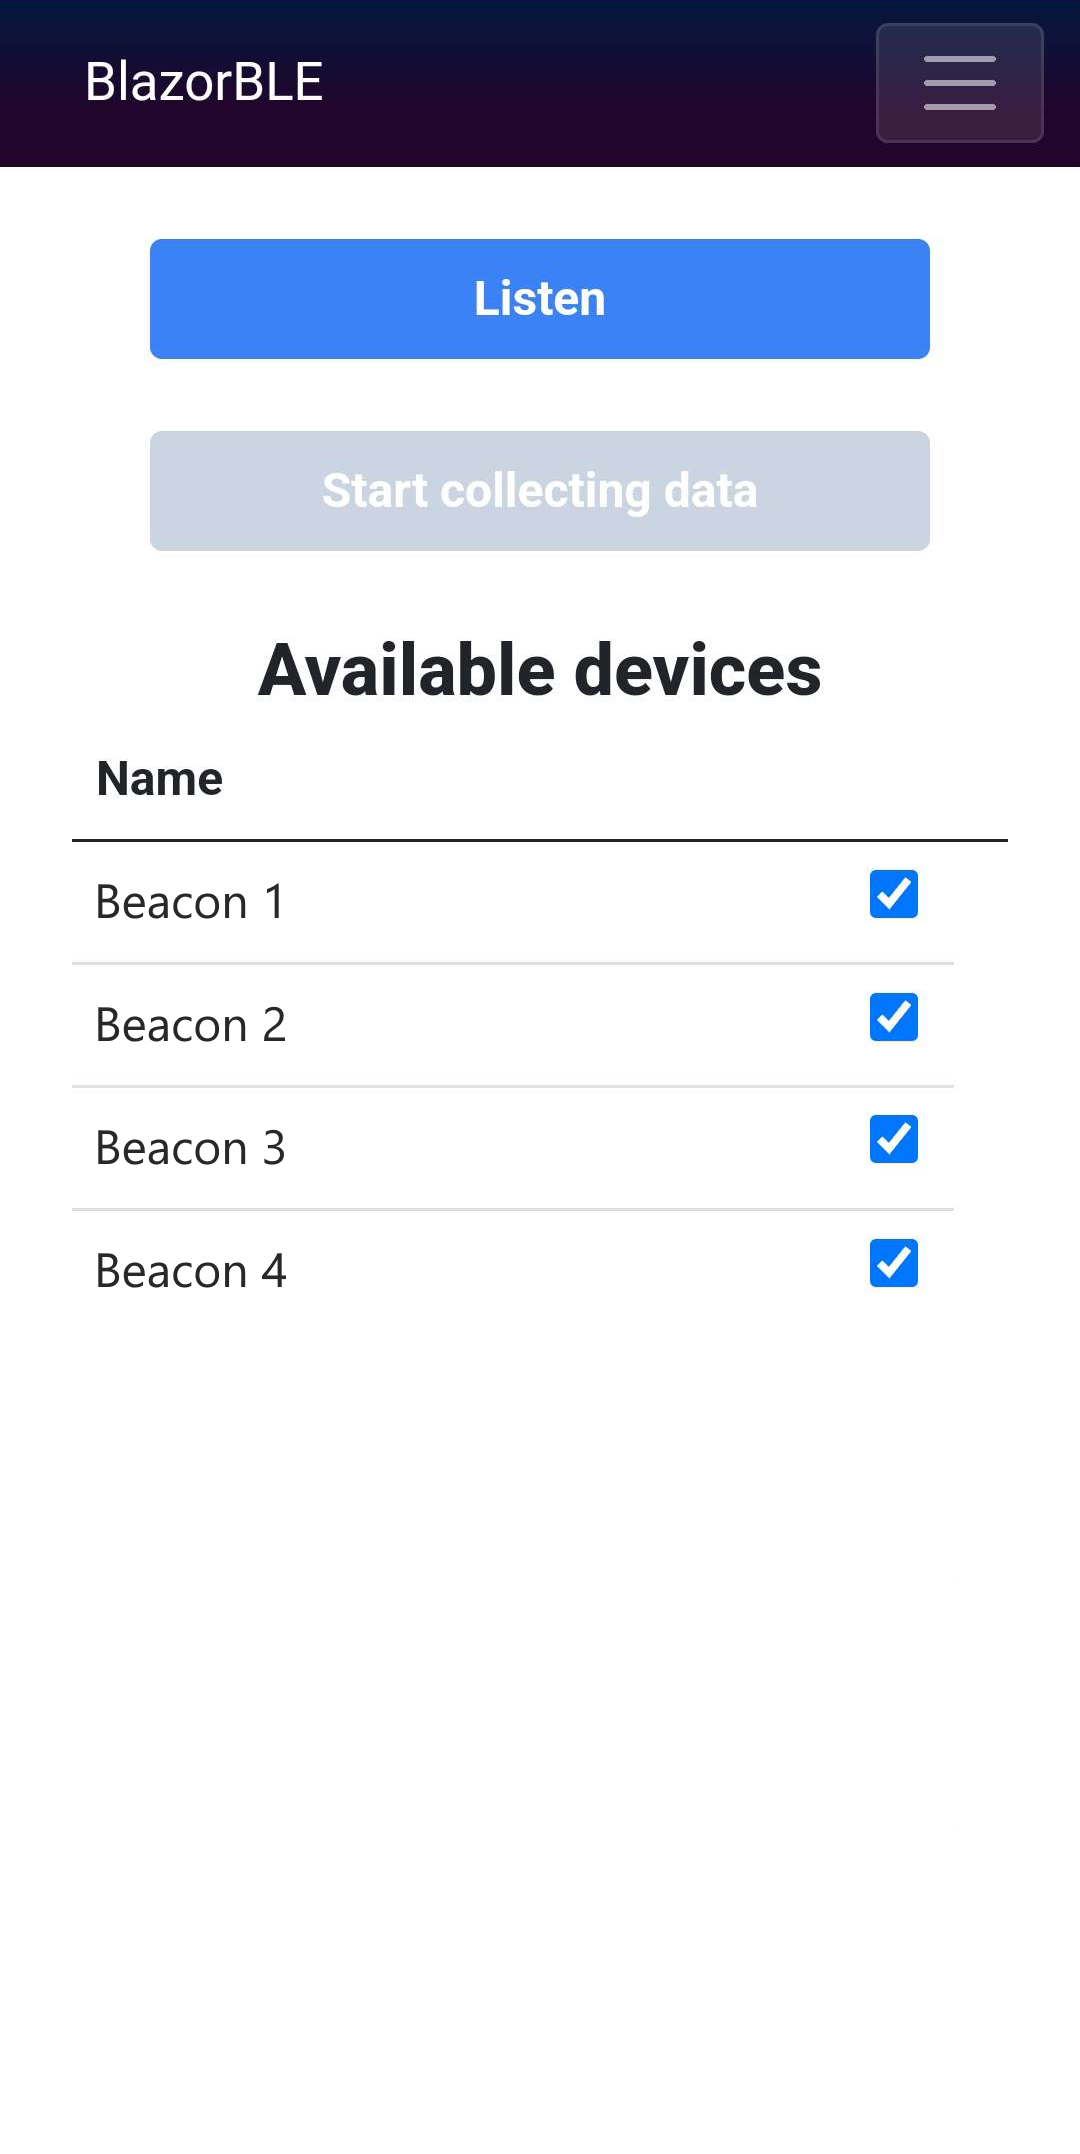
\includegraphics[width=\textwidth]{images/selected_devices.png}}
        \caption{Beacon selection view, showing BLE devices that broadcast iBeacon advertisement data.}
        \label{fig:selected_devices}
    \end{minipage}\hfill
    \begin{minipage}{0.41\textwidth}
        \centering
        \frame{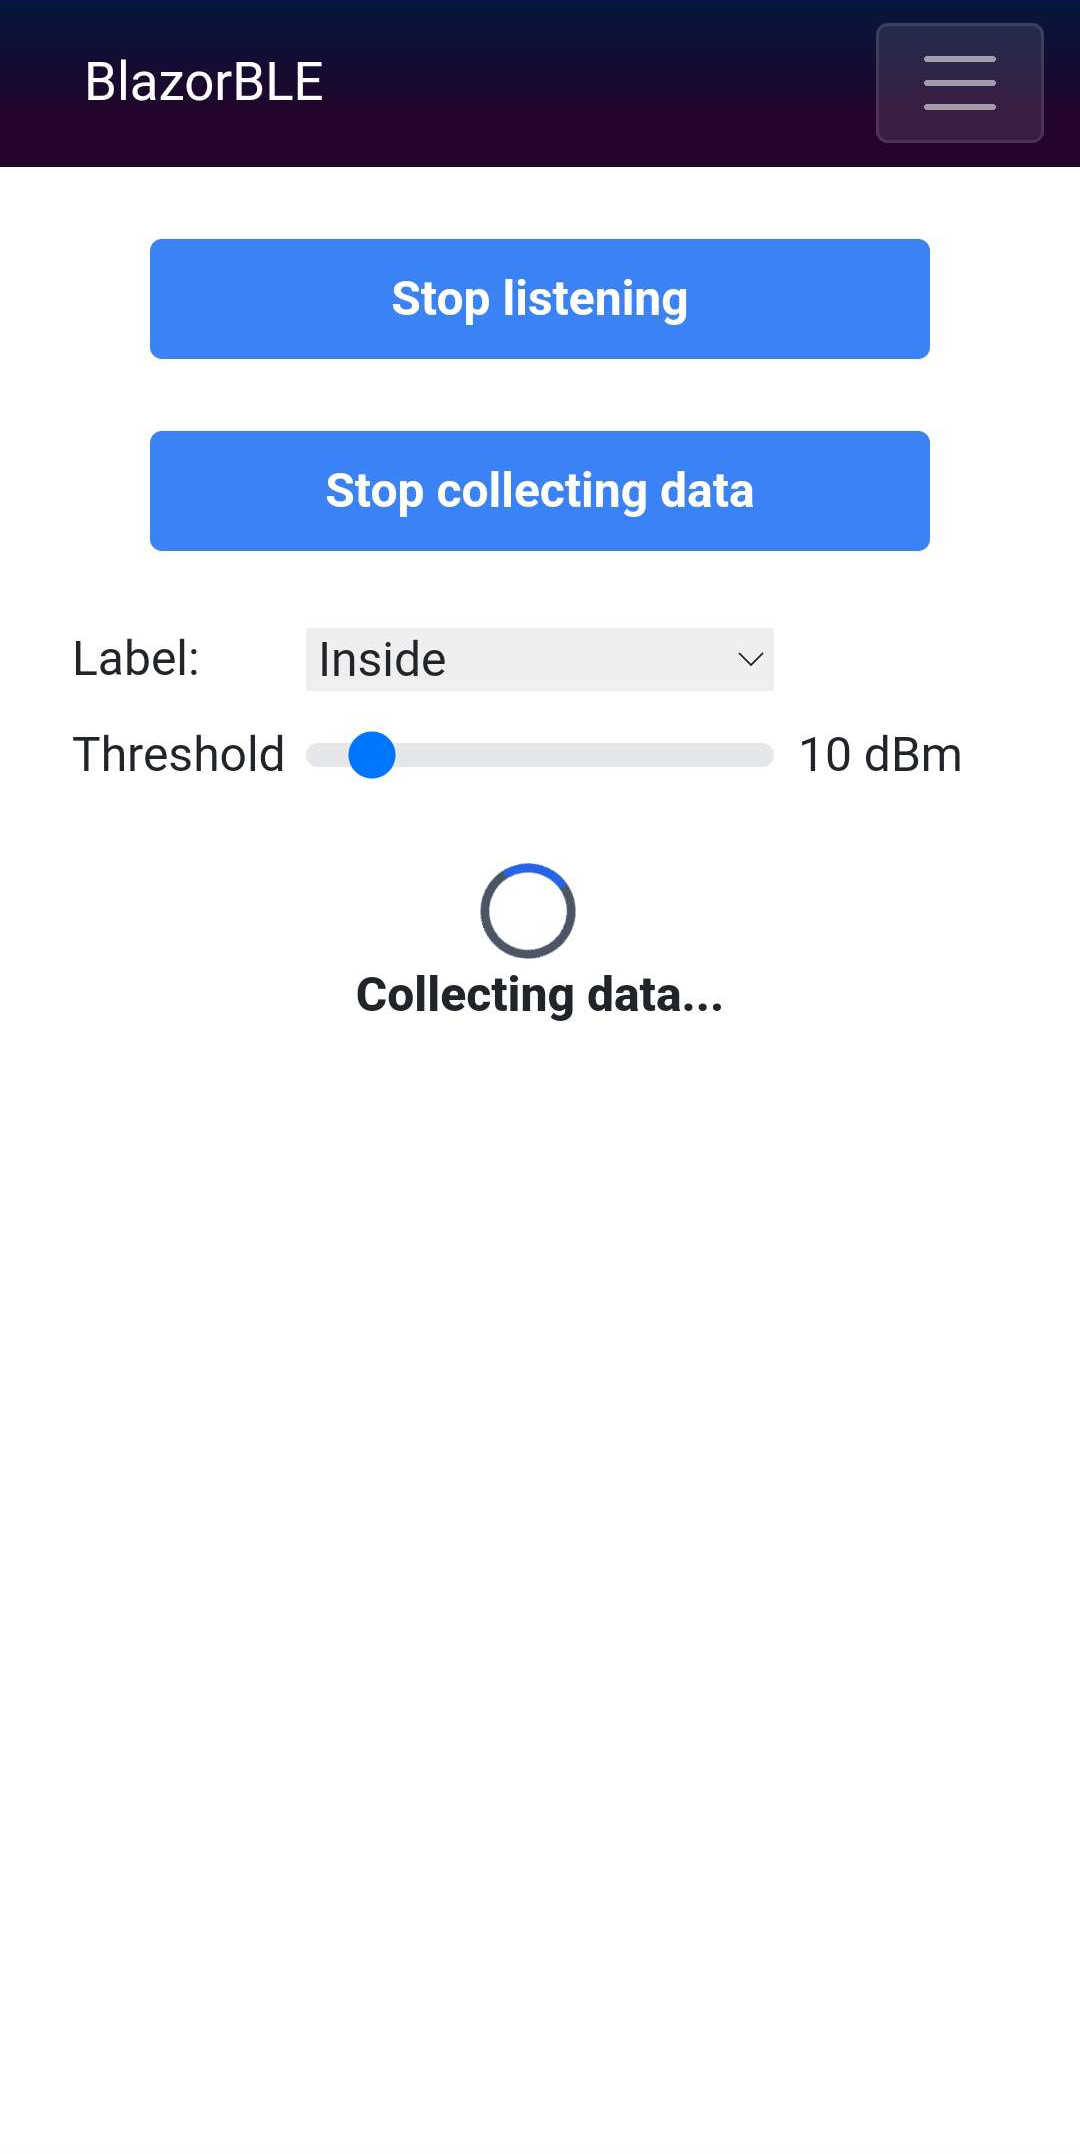
\includegraphics[width=\textwidth]{images/collecting_data.png}}
        \caption{The data collection view, showing that the user is collecting data, labelled as \textit{inside}.}
        \label{fig:collecting_data}
    \end{minipage}
\end{figure}
